%%%%%%%%%%%%%%%%%%%%%%%%%%%%%section Excitation signal setup %%%%%%%%%%%%%%%%%%%%%%%%%%%%%%%%%%%%%%%%%%%%%%%%%%%%%%%%%%%%
%%%%%%%%%%%%%%%%%%%%%%%%%%%%%%%%%%%%%%%%%%%%%%%%%%%%%%%%%%%%%%%%%%%%%%%%%%%%%%%%%%%%%%%%%%%%%%%%%%%%%%%%%%%%%%%%%%
\section{Excitation signal setup} \label{sec:FDTD_Excitation}
An excitation  is a source of the  electric magnetic field. It can be  an electrical field intensity $\vec{E}$ or an magnetic field intensity $\vec{H}$. And  in OpenEMS, each excitation can be considered as a composition  of two parts -- a signal of  time or  frequency as well as  a distribution or an application in the space. The first part is called excitation signal here. And in Matlab it is defined as one field of the structure \hyperref[para:FDTD]{\texttt{FDTD}}, which is named as \texttt{Excitation}. \phantomsection \label{para:Excitation}\\%\hyperref[para:Excitation]{\texttt{Excitation}} 

This section will show how to set up an \hyperref[para:Excitation]{\texttt{Excitation}} such as a Gaussian pulse, a sinusoidal signal or other customs excitation signals,\footnote{How to apply the \hyperref[para:Excitation]{\texttt{Excitation}}  to any given space(meshes or grids) is showed in the section \ref{sect-Primitives}.} with the following functions:
       \begin{myindentpar}
	      \hyperref[func:SetGaussExcite]{\texttt{SetGaussExcite(FDTD,f0,fc)}} \\ 
	      \hyperref[func:SetSinusExcite]{\texttt{SetSinusExcite(FDTD,f0)}}\\ 
	      \hyperref[func:SetCustomExcite]{\texttt{SetCustomExcite(FDTD,f0,funcStr)}}
       \end{myindentpar}
Note that Gaussian and sinusoidal excitatian are defined in frequency domain , since signals in time domain or frequency domain can be transformed into each other.   More Details are showed in the following subsections \ref{subsec:Gaussian pulse}, \ref{subsec:Sinousoidal signal} and \ref{subsec:Other excitation signals}\\
Exact definetion of these excitation signals can be found in the source codes file: \textasciitilde/openems/openEMS/FDTD/excitation.cpp.\\
\info{One  simulation has one excitation signal. 
And if many excitation signals are involved in a case, superposition principle can be utilized to  attain the equivalent simulation.}
%%%%%%%%%%%%%%%%%%%%%%%%%%%%%%%%%% subsection Gaussian pulse %%%%%%%%%%%%%%%%%%%%%%%%%%%%%%%%%%%%%%%%%%%%%%%%
    \subsection{Gaussian pulse} \label{subsec:Gaussian pulse}
If $f_0$ is a modulated frequency and $f_c$ is a bandwidth between  two cutoff frequencies $f_0-f_c/2$ and  $f_0+f_c/2$ at -5dB, then a time domain Gaussian signal (a pure Gaussian signal modulated by a co-sinusoidal signal)
\begin{equation}\label{equ:GussianSignal_time}
 f(t)=cos[2\pi f_0(t-t_0)]e^{-{\big(\frac{t-t_0}{\frac{t0}{3}}\big)}^2}, \quad \text{for } t>0 \text{ and }t_0=\frac{9}{2\pi f_c}
\end{equation}
can be expressed  in frequency domain as
\begin{equation}\label{equ:GussianSignal_freq}
F(f)=\frac{3}{4\sqrt{\pi}f_c}e^{-j\frac{9f}{f_c}}e^{-{\big(\frac{f-f_0}{\frac{2f_c}{3}}\big)}^2},\quad \text{for } f>0 .
\end{equation}

Figure \ref{fig:GaussInpulseTheory} shows an instance of Gaussian pulse from expressions \ref{equ:GussianSignal_time} and \ref{equ:GussianSignal_freq}. 
    \begin{figure}[hbt]
	      \centering
	      \subfloat[In time domain]{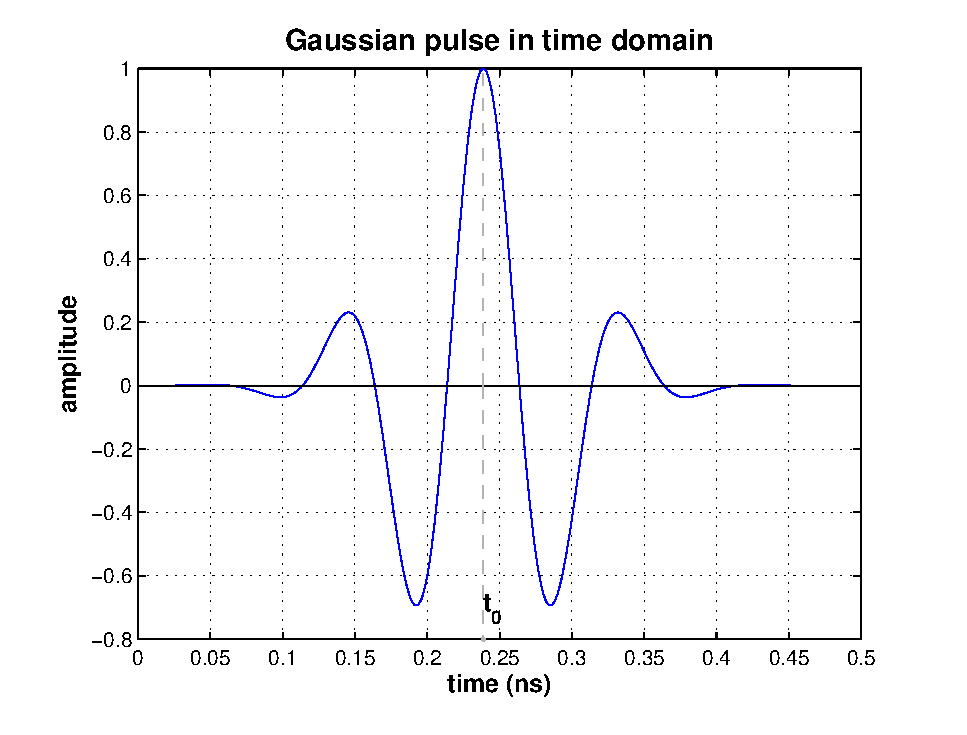
\includegraphics[width=0.48\textwidth]{svg/GaussPulseTime.eps}} 
	      \subfloat[In frequency domain]{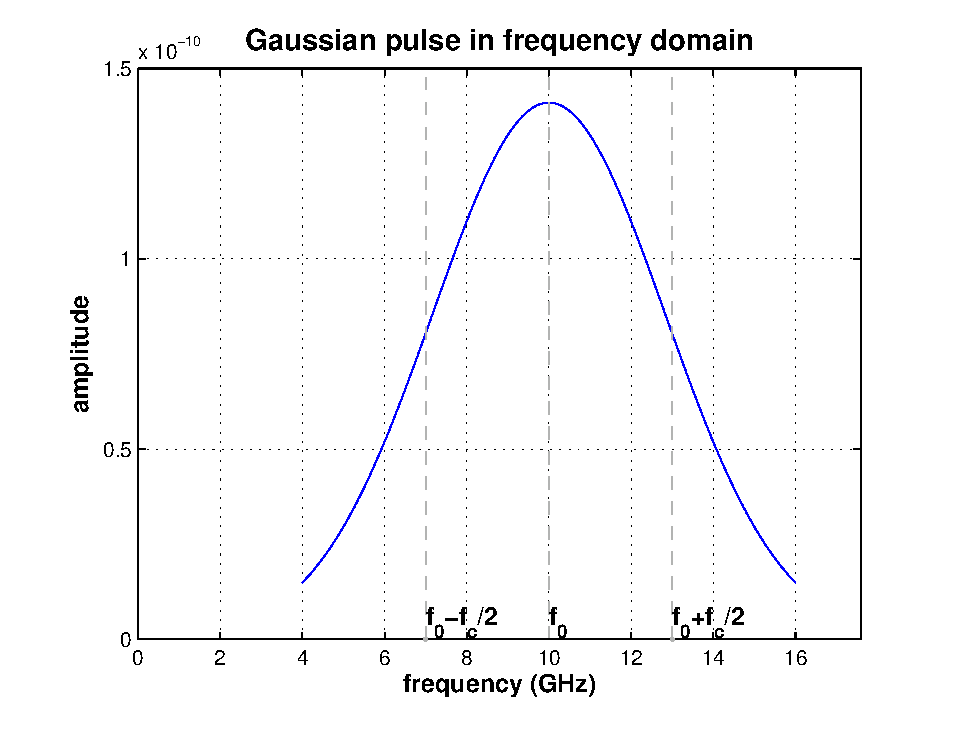
\includegraphics[width=0.48\textwidth]{svg/GaussPulseFreq.eps}}\\
	      \subfloat[In dB]{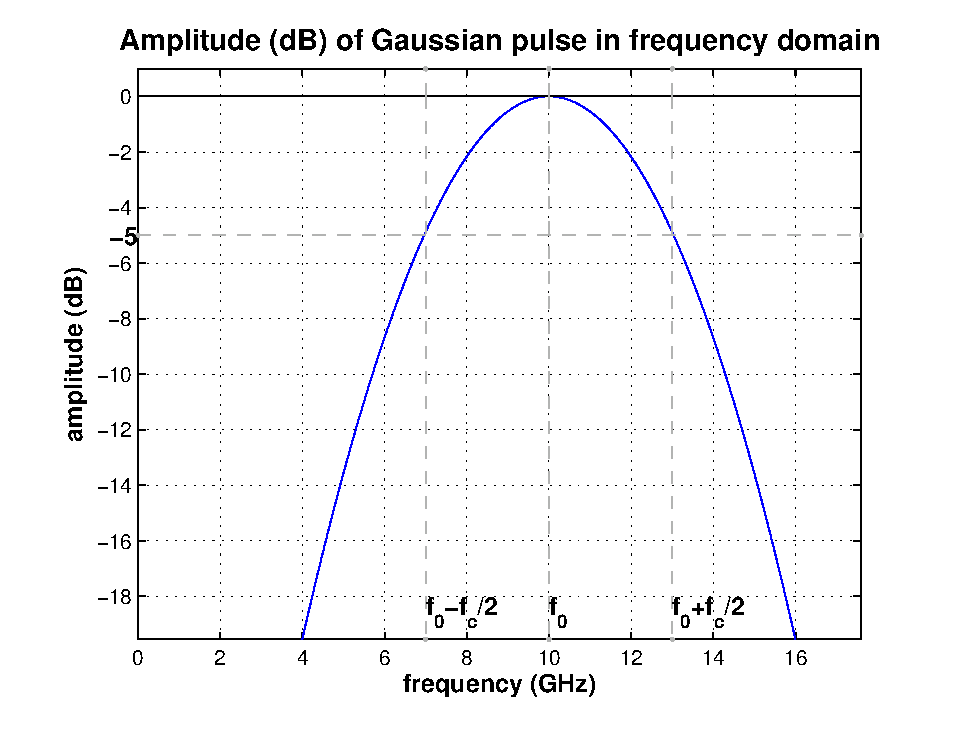
\includegraphics[width=0.48\textwidth]{svg/GaussPulseFreqdB.eps}} 
	      \caption[Gaussian pulse signal]{An instance of Gaussian pulse signal with $f_0=10GHz \quad f_c=6GHz$}
	      \label{fig:GaussInpulseTheory}
    \end{figure}
According to the expression \ref{equ:GussianSignal_freq}, a Gaussian signal can be defined with function \hyperref[func:SetGaussExcite]{\texttt{SetGaussExcite(FDTD,f0,fc)}}.

%%%%%%%%%%%%%%%%%%%%%%% FUNCTION  SetGaussExcite %%%%%%%%%%%%%%%%
\textcolor{blue}{\begin{large}\textbf{SetGaussExcite}	\end{large}}\phantomsection \label{func:SetGaussExcite}\\
	  Set a Gaussian function as the signal of the excitation.

\textcolor{blue}{\begin{large}Syntax:\end{large}}
 \begin{lstlisting}
FDTD = SetGaussExcite(FDTD,f0,fc)
 \end{lstlisting}

\textcolor{blue}{\begin{large}Definition:\end{large}}\\
      This function update the structure \hyperref[para:FDTD]{\texttt{FDTD}} with the expression \ref{equ:GussianSignal_freq}. 

\textcolor{blue}{\begin{large}Description:\end{large}}\\
%%%%%%%%%%%%%%%%%%%%%%%%%%%% FDTD
	\hyperref[para:FDTD]{\texttt{FDTD}} 
	    \begin{myindentpar}
		A structure in MATLAB. See \hyperref[para:FDTD]{\texttt{FDTD}}.
	    \end{myindentpar}
%%%%%%%%%%%%%%%%%%%%%%%%%%%% f0
	\texttt{f0}  \phantomsection \label{para:f0} %\hyperref[para:f0]{\texttt{f0}} 
	    \begin{myindentpar}
		\hyperref[para:f0]{\texttt{f0}}  is the frequency of the modulating co-sinusoidal signal. It's also the central frequency of the Gaussian signal. At this frequency the signal has the highest amplitude or energy. 
	    \end{myindentpar}
%%%%%%%%%%%%%%%%%%%%%%%%%%%% fc
	\texttt{fc}  \phantomsection \label{para:fc} %\hyperref[para:fc]{\texttt{fc}} 
	    \begin{myindentpar}
		\hyperref[para:fc]{\texttt{fc}} determines the variance of the signal. It is a central bandwidth. In the band [\hyperref[para:f0]{\texttt{f0}}-\hyperref[para:fc]{\texttt{fc}}/2 \quad \hyperref[para:f0]{\texttt{f0}}+\hyperref[para:fc]{\texttt{fc}}/2] the signal is greater then about -5dB. See figure \ref{fig:GaussInpulseTheory}. And the maximal frequency to be simulated is \hyperref[para:f0]{\texttt{f0}}+\hyperref[para:fc]{\texttt{fc}}.The greater \hyperref[para:fc]{\texttt{fc}} is, the flater is the signal in frequency domain, but cliffier and shorter in time domain.
	    \end{myindentpar}
\warning{Too small \hyperref[para:fc]{\texttt{fc}} will lead to a time-consuming simulation. Too great \hyperref[para:fc]{\texttt{fc}} will lead to a signal in a very short time relative to a time step. Both cases should be advoided.}

%%%%%%%%%%%%%%%%%%%%% Examples.	  
	\textcolor{blue}{\begin{large}Examples:\end{large}}\\
\begin{itemize}
\item An Gaussian pulse with a central frequency \hyperref[para:f0]{\texttt{f0}}=0.5GHz, and a -5dB bandwidth of \hyperref[para:fc]{\texttt{fc}}=0.5GHz. 
\begin{lstlisting}
% Initiation of FDTD 
FDTD = InitFDTD(5000,1e-5,'OverSampling',10);
% Update FDTD with a  Gaussian pulse excitation. 
% f0=0.5GHz, fc=0.5GHz
FDTD = SetGaussExcite(FDTD,0.5e9,0.5e9);
% The field  FDTD.Excitation.ATTRIBUTE  has been assigned.
\end{lstlisting}
Under this setting, a Gaussian pulse has been set up. And the signal reduces to -5dB at 0.25GHz and 0.75GHz. The maximal frequency in simulation is 1GHz.
\end{itemize}

%%%%%%%%%%%%%%%%%%%%%%%%%%%%%%%%%%%% subsection Sinousoidal signal %%%%%%%%%%%%%%%%%%%%%%%%%%%%%%%%%%%%%%%%%%%%%%%%%%%%%%%%%%%%%%%%%%%%%
    \subsection{Sinousoidal signal}\label{subsec:Sinousoidal signal}
\textcolor{blue}{\begin{large}\textbf{SetSinusExcite}	\end{large}}\phantomsection \label{func:SetSinusExcite}\\
	  Set a sinusoidal function as the signal of the excitation.

\textcolor{blue}{\begin{large}Syntax:\end{large}}
 \begin{lstlisting}
FDTD = SetSinusExcite(FDTD,f0)
 \end{lstlisting}

\textcolor{blue}{\begin{large}Definition:\end{large}}\\
      The signal in time domain has an form as following function\\
\begin{equation}\label{equ:SinusoidalSignal_time}
 f(t)=\sin{(2\pi f_0t)}, \text{ for } t>0
\end{equation}

\textcolor{blue}{\begin{large}Description:\end{large}}\\
%%%%%%%%%%%%%%%%%%%%%%%%%%%% FDTD
	\hyperref[para:FDTD]{\texttt{FDTD}} 
	    \begin{myindentpar}
		A structure in MATLAB interface. See \hyperref[para:FDTD]{\texttt{FDTD}}.
	    \end{myindentpar}
%%%%%%%%%%%%%%%%%%%%%%%%%%%% f0
	\texttt{f0}  \phantomsection \label{para:sin_f0} %\hyperref[para:sin_f0]{\texttt{f0}} 
	    \begin{myindentpar}
		\hyperref[para:sin_f0]{\texttt{f0}}  is the unique frequency of the homonic signal. 
	    \end{myindentpar}

%%%%%%%%%%%%%%%%%%%%% Examples.	  
	\textcolor{blue}{\begin{large}Examples:\end{large}}\\
\begin{itemize}
\item A sinousoidal signal with a  frequency \hyperref[para:sin_f0]{\texttt{f0}}=0.5GHz. 
\begin{lstlisting}
% Initiation of FDTD 
FDTD = InitFDTD(5000,1e-5,'OverSampling',10);
% Assignment for f0
f0=0.5e9;
% Update FDTD with a sinousoidal excitation. 
FDTD = SetSinusExcite(FDTD,f0);
% The field  FDTD.Excitation.ATTRIBUTE
% has been assigned.
\end{lstlisting}
A sinousoidal excitation with frequency 0.5GHz has been set up in OpenEMS. 
\end{itemize}

%%%%%%%%%%%%%%%%%%%%%%%%%%%%%%%%%%%% subsection excitation signals %%%%%%%%%%%%%%%%%%%%%%%%%%%%%%%%%%%%%%%%%%%%%%%%%%%%%%%%%%%%%%%%%%%%%
    \subsection{Other excitation signals}\label{subsec:Other excitation signals}
OpenEMS provides various kinds of excitation signals. Besides the Gaussian pulse and sinusoidal signal, it has also other forms of excitation, such as dirac function, step function and even custom function. Here is the introduction of how to set up an excitation with any custom function by using \hyperref[func:SetCustomExcite]{\texttt{SetCustomExcite}}.

\textcolor{blue}{\begin{large}\textbf{SetCustomExcite}	\end{large}}\phantomsection \label{func:SetCustomExcite}\\
	  Set a custom function as the signal of the excitation.

\textcolor{blue}{\begin{large}Syntax:\end{large}}
 \begin{lstlisting}
FDTD = SetCustomExcite(FDTD,f0,funcStr)
 \end{lstlisting}

\textcolor{blue}{\begin{large}Definition:\end{large}}\\
      The signal in time domain is a function like the given string \texttt{funcStr}.

\textcolor{blue}{\begin{large}Description:\end{large}}\\
%%%%%%%%%%%%%%%%%%%%%%%%%%%% FDTD
	\hyperref[para:FDTD]{\texttt{FDTD}} 
	    \begin{myindentpar}
		A structure in MATLAB. See \hyperref[para:FDTD]{\texttt{FDTD}}.
	    \end{myindentpar}
%%%%%%%%%%%%%%%%%%%%%%%%%%%% f0
	\texttt{f0}  \phantomsection \label{para:custom_f0} %\hyperref[para:f0]{\texttt{f0}} 
	    \begin{myindentpar}
		\hyperref[para:f0]{\texttt{f0}}  is the nyquist rate. 
	    \end{myindentpar}
%%%%%%%%%%%%%%%%%%%%%%%%%%%% funcStr
	\texttt{funcStr}  \phantomsection \label{para:custom_funcStr} %\hyperref[para:custom_funcStr]{\texttt{funcStr}} 
	    \begin{myindentpar}
		\hyperref[para:custom_funcStr]{\texttt{funcStr}}   is a string of an expression in MATLAB. This expression is of \texttt{t}, the time. It denotes how is the function of excitation.  And two constants can be used directly in the expression, \texttt{e} for Euler's number and \texttt{pi} for $\pi$. Futher more any strings of defined valuables can be used in \hyperref[para:custom_funcStr]{\texttt{funcStr}}.
	    \end{myindentpar}

%%%%%%%%%%%%%%%%%%%%% Examples.	  
	    \textcolor{blue}{\begin{large}Examples:\end{large}}\\
    \begin{itemize}
	\item A ramped sinus excite 
	\begin{lstlisting}
% Initiation of FDTD 
FDTD = InitFDTD(5000,1e-5,'OverSampling',10);
% The nyquist rate f0=1GHz
f0=1e9;
% Time step is of the nyquist rate f0
T = 1/f0;
% Update FDTD with a given string 
% of an excitation expression of t. 
FDTD = SetCustomExcite(FDTD,f0, ...
       [ '(1-exp(-1*(t/' num2str(T) ...
        ')^2) ) * sin(2*pi*'  ...
        num2str(f0) '*t)' ]);
% The field  FDTD.Excitation.ATTRIBUTE 
% has  been assigned.
	\end{lstlisting}
    \end{itemize}
